\documentclass[12pt,spanish]{article}
\usepackage[spanish,es-tabla]{babel}
\usepackage[utf8]{inputenc}
\usepackage[normalem]{ulem}	
\usepackage{lmodern}
\usepackage{rotating}
\usepackage{ragged2e}
\usepackage{natbib}
\usepackage{amsmath}
\usepackage{graphicx}
\usepackage{subcaption}
\usepackage{booktabs}
\usepackage{hyperref}
\usepackage{wrapfig} 
\usepackage{listings}
\usepackage{listingsutf8}
\usepackage{subfigure}
\usepackage{subcaption}
\usepackage{longtable}
\usepackage{graphics}
\usepackage{graphicx}
\usepackage{parskip}
\usepackage{amsmath}
\usepackage{amssymb}
\usepackage{amsthm}
\usepackage{float}
\usepackage{caption}
\usepackage{multicol}
\usepackage{pdfpages}
\usepackage{textcomp}
\usepackage{hyperref}
\usepackage{tikz}
\usetikzlibrary{shapes,arrows,spy,positioning,snakes}
\usepackage{caption}
\usepackage{xcolor}	%Paquete para colores
\usepackage{color}	%Colores
\usepackage{colortbl}
\usepackage{indentfirst}
\usepackage{enumerate} 
\usepackage{shapepar}
\usepackage{anysize} 
\usepackage{fancyvrb}
\usepackage{stackrel}
\usepackage{amsfonts}
\usepackage{framed}
\usepackage{float}
\spanishdecimal{.}
\definecolor{shadecolor}{rgb}{0.6,1,0.5}
\DeclareGraphicsExtensions{.pdf,.png,.jpg}
\usepackage[rmargin=2cm,lmargin=1cm,top=2cm,bottom=2cm]{geometry}  
\usepackage{setspace}
\usepackage{booktabs}
\spanishdecimal{.}
\usepackage{xcolor}
\usepackage{appendix}
\renewcommand{\appendixpagename}{Anexos}
\renewcommand{\appendixtocname}{Anexos}
\definecolor{grannysmithapple}{rgb}{0.66, 0.89, 0.63}
\definecolor{codegreen}{rgb}{0,0.6,0}
\definecolor{codered}{rgb}{0.5,0.5,0.5}
\definecolor{codepurple}{rgb}{0.58,0,0.82}
\definecolor{backcolour}{rgb}{0.95,0.95,0.92}

\lstdefinestyle{mystyle}{
    backgroundcolor=\color{backcolour},   
    commentstyle=\color{cyan},
    keywordstyle=\color{red},
    numberstyle=\tiny\color{codepurple},
    stringstyle=\color{brown},
    basicstyle=\ttfamily\footnotesize,
    breakatwhitespace=false,         
    breaklines=true,                 
    captionpos=b,                    
    keepspaces=true,                 
    numbers=left,                    
    numbersep=5pt,                  
    showspaces=false,                
    showstringspaces=false,
    showtabs=false,                  
    tabsize=2
}
\lstset{style=mystyle}
\parindent=0cm

\usepackage{dcolumn}
\newcolumntype{2}{D{.}{}{2.0}}
\usepackage{tikz}
\usetikzlibrary{positioning}
\definecolor{offwhite}{HTML}{000000}
\tikzset{
    > = stealth,
    every node/.append style = {
        text = offwhite
    },
    every path/.append style = {
        arrows = ->,
        draw = offwhite,
        fill = offwhite
    },
    hidden/.style = {
        draw = offwhite,
        shape = circle,
        inner sep = 1pt
    },
    square/.style = {
        draw = offwhite,
        thick,
        rectangle,
        minimum size = 12pt,
        inner sep = 5pt
    }
}

\title{Reporte SAE y Modelos mixtos}
\author{Luz Elenis Torres Bertel}
\date{}

\begin{document}

\maketitle

\section*{Estimación en áreas pequeñas SAE}

Cuando se realizan estimaciones directas en una muestra, el objetivo principal es encontrar estimaciones fiables para la población, para algunos subgrupos o conjuntos en específico de la misma, de esta forma nace el problema de cuando se quieren estudiar dominios o áreas específicas que el diseño de la encuesta no contempló o en el que el tamaño de la muestra de dicho dominio es insuficiente, es así como SAE es un método alternativo para obtener estimaciones precisas en estos casos.

Las técnicas estadísticas de SAE se dividen en tres grupos: métodos basados en diseño, métodos asistidos por modelos y métodos basados en modelos. Estas técnicas buscan estimadores que compitan con los estimadores directos.  

\begin{itemize}
    \item \textbf{métodos basados en diseño:}
    Los métodos basados en diseño usan información externa para crear estimadores indirectos que pueden ser más precisos que los directos, sin depender explícitamente de modelos. Por ejemplo, si se tiene información de la población por sexo y edad, se puede usar para mejorar las estimaciones.
    \item \textbf{métodos asistidos por modelos:}
    La metodología asistida por modelos usa modelos explícitos para elegir estimadores, considerando sus propiedades bajo la distribución basada en el diseño. Ejemplos importantes son el estimador de regresión generalizada (GREG), el estimador de calibración y el estimador LGREG. El estimador GREG utiliza un modelo lineal para estimar la media de una variable continua y está diseñado para ser insesgado, independientemente de cómo se ajuste el modelo a los datos.
    \item \textbf{métodos basados en modelos:}
    El enfoque basado en modelos asume que los datos provienen de un modelo verdadero y usa modelos explícitos para combinar diferentes fuentes de información. Este enfoque puede usar información auxiliar y considerar correlaciones temporales y espaciales, produciendo estimadores con propiedades óptimas. Es crucial seleccionar y diagnosticar bien el modelo para obtener buenos estimadores con errores menores. 
\end{itemize}

Los modelos de área pequeña se dividen en dos grupos: a nivel de unidad y a nivel de área. El modelo de regresión de errores anidados (NER) es un ejemplo de modelo a nivel de unidad, usado para predecir áreas de cultivo en EE.UU. Los mejores predictores empíricos (EBLUP) basados en NER se usan ampliamente. 

El modelo de Fay-Herriot (FH) es un ejemplo de modelo a nivel de área, usado para estimar ingresos per cápita en EE.UU. Este modelo y sus variantes se han aplicado a la estimación de la pobreza en España y otros lugares, usando modelos mixtos lineales y generalizados.

\section*{Modelos Lineales Mixtos}

Los modelos lineales (LM) asumen que todas las observaciones son independientes y vienen de la misma población. Los modelos mixtos, por otro lado, consideran que las observaciones en diferentes niveles o conglomerados son independientes, pero las observaciones dentro del mismo nivel o conglomerado se consideran dependientes porque comparten característocas. Para estos datos, podemos hablar de dos fuentes de variación: entre y dentro de los clústeres, lo que les permite manejar datos más complejos.

Los modelos lineales mixtos (LMM) son útiles cuando las observaciones no son independientes, ya que pueden corregir errores correlacionados. Los GLMM son una extensión de los LMM para variables que no siguen una distribución normal, permitiendo predicciones más precisas.

Estos modelos son muy flexibles y pueden combinar diferentes fuentes de información, lo que los hace ideales para la estimación de áreas pequeñas. Incorporan efectos fijos y aleatorios para manejar datos repetidos y correlaciones espaciales y temporales. Estos modelos son particularmente útiles cuando se trabaja con datos que tienen una estructura jerárquica o agrupada.

La forma general de un modelo lineal mixto se puede expresar como:

$$y = X\beta + Zu + \epsilon$$

Donde:
\begin{itemize}
    \item $y$ es el vector de variables respuesta
    \item $X$ es la matriz de diseño para los efectos fijos
    \item $\beta$ es el vector de coeficientes de efectos fijos
    \item $Z$ es la matriz de diseño para los efectos aleatorios
    \item $u$ es el vector de efectos aleatorios
    \item $\epsilon$ es el vector de errores residuales
\end{itemize}

\begin{align*}
\text{var}(u) &= E[\text{uu}'] = V_u, \\
\text{var}(e) &= E[\text{ee}'] = V_e,
\end{align*}

dependiendo de un parámetro \(\sigma\) que contiene los componentes de varianza. 

\[
V = \text{var}(y) = ZV_uZ' + V_e,
\]

donde se asume que \(V\) no es singular.

La estimación por mínimos cuadrados para beta sera:

$$\hat{\beta} = (X^T V^{-1} X)^{-1} X^T V^{-1} y
$$

La estimación de los mejores predictores empíricos lineales no sesgados $BLUP$ para $u$ bajo el modelo es:

$$\hat{u} = V_u Z' V^{-1} (y - X\beta)
$$
\subsection*{¿Cómo funciona el EBLUP (Empirical Best Linear Unbiased Predictor)?}

Como se mencionó anteriormente el \textbf{EBLUP} se usa cuando se tiene información a nivel de unidad(individuos) y de área(grupos). Es un método de mucha ayuda para predecir el valor de la variable que se quiera estudiar para una unidad particular combinando información general como los efectos fijos e información más específica como los efectos aleatorios.

\textbf{Siglas:}

\begin{itemize}
    \item Empirical:las estimaciones de los parámetros del modelo se hacen a partir de los datos
    \item Best: Es el mejor porque es el que más minimiza el error cuadrático medio
    \item Linear: Es una combinación linal de los datos observados
    \item Unbiased: las predicciones no presentan sesgo en promedio 
\end{itemize}

El \textbf{EBLUP} se obtiene en dos pasos: primero se estiman los parámetros del modelo y después se calculan las predicciones de los efectos aleatorios y la variable dependiente

\begin{enumerate}
    \item Primero se estiman los parámetros del modelo, con la notación anterior: $\beta$ (Coeficientes de los efectos fijos) $V_u$ (varianza de los efectos aleatorios), $V_e$ (varianza residual)
    \item segundo, Se procede a calcular el EBLUP para los efectos aleatorios $u$, como se mencionó anteriormente esta estimación será: 

\[
\hat{u} = V_u Z' V^{-1} (y - X\beta)
\]
\end{enumerate}

Donde:
\begin{itemize}
    \item $\hat{u}$ es la predicción del efecto aleatorio en los grupos
    \item $V_u$ es la matriz de varianza de los efectos aleatorios $\hat{u}$
    \item $Z$ es la matriz de diseño de los efectos aleatorios
    \item $V$ es la matriz de varianza de los errores de predicción para los grupos
    \item $y$ el vector de datos observados
    \item $X$ y $\beta$ son la matriz de diseño y el vector de coeficientes estimados para los efectos fijos
\end{itemize}

\textbf{Ventajas:}

El EBLUP, o mejor estimador lineal insesgado de predicción, es una técnica estadística avanzada que ofrece varias ventajas en el análisis de datos. Su capacidad para combinar efectos fijos y aleatorios permite una interpretación más rica y detallada de los datos, especialmente útil en estudios que involucran múltiples grupos o categorías. Además, al incorporar información de la estructura del modelo y datos específicos, el EBLUP reduce la varianza de las estimaciones, lo que resulta en predicciones más precisas y confiables. Esta precisión es particularmente valiosa en la estimación en áreas pequeñas, donde los tamaños de muestra reducidos pueden hacer que otros métodos sean menos fiables. Por lo tanto, el EBLUP se convierte en una herramienta indispensable para investigadores y analistas que buscan maximizar la información extraída de sus datos, especialmente en contextos donde las observaciones son limitadas.

\subsection*{Componentes y supuestos de los Modelos Lineales Mixtos}

\subsubsection*{ Efectos Fijos}

Los efectos fijos ($X\beta$) son parámetros asociados con una población entera o con ciertos niveles reproducibles de factores experimentales. Se asume que estos efectos son constantes y se estiman directamente.

\subsubsection*{Efectos Aleatorios}

Los efectos aleatorios ($Zu$) son variables aleatorias asociadas con unidades de muestreo extraídas al azar de una población. Se asume que estos efectos siguen una distribución (generalmente normal) con media cero y una cierta matriz de varianza-covarianza.

\subsubsection*{Errores Residuales}

Los errores residuales ($\epsilon$) representan la variabilidad no explicada por los efectos fijos y aleatorios. Se asume que son independientes y siguen una distribución normal con media cero y varianza constante.

\subsubsection*{Supuestos:}

Los modelos lineales mixtos (MLM) se basan en los siguientes supuestos clave:

\begin{enumerate}
    \item Linealidad: La relación entre las variables predictoras y la respuesta es lineal.
    \item Normalidad: Los efectos aleatorios y los errores residuales siguen una distribución normal.
    \item Homocedasticidad: La varianza de los errores es constante.
    \item Independencia: Los errores son independientes entre sí.
    \item Los efectos aleatorios son independientes de los errores residuales.
\end{enumerate}

\section*{Modelos de Fay-Herriot}

Los modelos a nivel de unidad son útiles para describir una variable objetivo si se ajustan bien a los datos. Para calcular los mejores predictores lineales no sesgados (EBLUPs) bajo un modelo mixto lineal a nivel de unidad, se necesita un archivo con los promedios de las variables auxiliares. Esto limita las variables disponibles y reduce la precisión del modelo. Además, los datos agregados de registros administrativos pueden no coincidir exactamente con los datos de la encuesta.

Para calcular los mejores predictores empíricos (PBE) de parámetros no lineales, se necesita un archivo censal con las variables auxiliares, lo cual es complicado para muchas oficinas de estadística. Si las variables auxiliares son categóricas, se pueden usar los tamaños de población por categorías, pero esto no siempre es suficiente para predecir la variable objetivo.

Estos problemas son comunes en la estimación de áreas pequeñas (SAE). Si no hay buena información individual, pero sí datos agregados, se puede usar un modelo a nivel de área. El modelo de Fay y Herriot (1979) es un ejemplo de modelo a nivel de área usado para estimar ingresos en pequeños lugares de EE.UU. y es uno de los más utilizados para la estimación de áreas pequeñas.

Los EBLUP basados en el modelo de Fay-Herriot tienen la desventaja de perder información al agregar datos a nivel de unidad. Sin embargo, tienen varias ventajas:

\begin{enumerate}
    \item Pueden usar más variables auxiliares.
    \item No necesitan que las mismas variables auxiliares estén en la encuesta y en los registros administrativos.
    \item Funcionan bien cuando hay muchas áreas pequeñas con tamaños de muestra pequeños.
\end{enumerate}

El modelo de Fay-Herriot ha sido ampliamente investigado y aplicado en muchos campos diferentes.

\subsection*{El modelo de Fay-Herriot a nivel de área}

El modelo Fay--Herriot de nivel de área consta de dos etapas. En la primera etapa, un modelo de muestreo se utiliza para representar el error de muestreo de estimadores directos. Sea \(\mu_d\) la característica de interés en el área \(d\)-ésima y \(y_d\) un estimador directo de \(\mu_d\). En aplicaciones a datos reales, \(\mu_d\) es típicamente la media del dominio:

\[
\mu_d = \frac{1}{N_d} \sum_{j=1}^{N_d} y_{dj},
\]

donde \(y_{dj}\) es la variable objetivo medida a nivel unitario. El modelo de muestreo indica que los estimadores directos \(y_d\) son insesgados y se pueden expresar como:

\[
y_d = \mu_d + e_d, \quad d = 1, \dots, D,
\]

donde \(D\) es el número total de áreas o dominios. Aquí, \(e_d\) representa errores de muestreo que son independientes y normalmente distribuidos con varianzas conocidas:

\[
e_d \sim N(0, \sigma^2_{e_d}),
\]

donde \(\sigma^2_{e_d}\) es la varianza basada en el diseño del estimador directo \(y_d\). En la segunda etapa, se asume que las verdaderas características del área \(\mu_d\) varían linealmente con \(p\) variables auxiliares de nivel de área:

\[
\mu_d = \mathbf{x}_d\beta + u_d, \quad d = 1, \dots, D,
\]

donde \(\mathbf{x}_d\) es un vector fila con los valores agregados de \(p\) variables auxiliares para el área \(d\), \(\beta\) es el vector columna de coeficientes de regresión, y \(u_d\) son errores de modelo, típicamente distribuidos como \(u_d \sim N(0, \sigma^2_u)\) con varianza \(\sigma^2_u\) desconocida e independiente de \(e_d\). Este modelo, llamado modelo de vinculación, conecta las verdaderas medias de todas las áreas a través del parámetro de regresión común \(\beta\).

El modelo Fay--Herriot puede expresarse en una única forma:

\[
y_d = \mathbf{x}_d\beta + u_d + e_d, \quad d = 1, \dots, D.
\]

o en notación matricial:

\[
\mathbf{y} = \mathbf{X}\beta + \mathbf{Z}\mathbf{u} + \mathbf{e},
\]

donde \(\mathbf{Z} = \mathbf{I}_D\) y \(\mathbf{I}_D\) es una matriz diagonal de identidad.

\section*{Modelo bayesiano de Fay-Herriot}

El modelo bayesiano de Fay-Herriot es una extensión jerárquica bayesiana (HB) para predecir medias de dominio en modelos de nivel de área. El modelo combina observaciones directas con información auxiliar disponible para mejorar las estimaciones en dominios con muestras limitadas.

\subsection*{Modelo Jerárquico}

El modelo de Fay-Herriot se estructura en dos niveles:

\subsection*{Nivel de Muestreo (Modelo de Observación)}

Para cada área \( d \), se tiene una observación directa \( y_d \) que es una estimación ruidosa de la verdadera media del dominio \( \mu_d \):

\begin{equation*}
    y_d = \mu_d + e_d, \quad e_d \sim N(0, \sigma^2_d),
\end{equation*}

donde \( e_d \) es el error de muestreo, que sigue una distribución normal con varianza \( \sigma^2_d \), conocida para cada área.

\subsection*{Nivel de Área (Modelo Estructural)}

La verdadera media \( \mu_d \) se modela como una función de covariables \( x_d \) y un efecto aleatorio \( u_d \):

\begin{equation*}
    \mu_d = x_d' \beta + u_d, \quad u_d \sim N(0, \sigma^2_u),
\end{equation*}

donde:
\begin{itemize}
    \item \( x_d \) es un vector de covariables para el área \( d \),
    \item \( \beta \) es el vector de coeficientes de regresión,
    \item \( u_d \) es el efecto aleatorio, que sigue una distribución normal con media 0 y varianza \( \sigma^2_u \).
\end{itemize}

\section*{Perspectiva Bayesiana}

Desde la perspectiva bayesiana, se colocan distribuciones a priori sobre los parámetros desconocidos:

\begin{itemize}
    \item Para \( \beta \), se asume una distribución a priori no informativa: \( f_0(\beta) = 1 \).
    \item Para \( \sigma^2_u \), se puede asumir una distribución a priori gamma inversa, facilitando la estimación bayesiana de \( \sigma^2_u \).
\end{itemize}

\section*{Predicción Bayesiana}

El objetivo es predecir la verdadera media \( \mu_d \) de cada dominio mediante la media posterior:

\begin{equation*}
    \mu_d^{HB} = E[\mu_d | y].
\end{equation*}

Bajo el modelo de Fay-Herriot, el predictor bayesiano jerárquico es una combinación ponderada de la observación directa \( y_d \) y la predicción basada en las covariables \( x_d \):

\begin{equation*}
    \mu_d^{HB} = \frac{\sigma^2_u}{\sigma^2_u + \sigma^2_d} y_d + \frac{\sigma^2_d}{\sigma^2_u + \sigma^2_d} x_d' \hat{\beta}.
\end{equation*}

\subsection*{Varianza Posterior}

La varianza posterior de \( \mu_d \) está dada por:

\begin{equation*}
    \text{var}(\mu_d | y) = \frac{\sigma^2_d \sigma^2_u}{\sigma^2_d + \sigma^2_u} + \frac{\sigma^4_d}{(\sigma^2_d + \sigma^2_u)^2} x_d' V_{\beta} x_d,
\end{equation*}

donde \( V_{\beta} \) es la matriz de covarianzas de los coeficientes \( \beta \).

\section*{Estimación de \( \sigma^2_u \)}

El parámetro \( \sigma^2_u \) no es conocido, por lo que puede estimarse de dos formas:

\begin{itemize}
    \item \textbf{Bayes Empírico}: Se estima \( \sigma^2_u \) a partir de los datos utilizando métodos como la máxima verosimilitud restringida (REML).
    \item \textbf{Bayes Completo}: Se utiliza una distribución a priori para \( \sigma^2_u \) (por ejemplo, una gamma inversa), y se aplica muestreo MCMC, como el algoritmo de Gibbs.
\end{itemize}

\section*{Muestreo de Gibbs}

Cuando \( \sigma^2_u \) no es conocido y se utiliza el enfoque bayesiano completo, los parámetros del modelo se pueden estimar usando el algoritmo de Gibbs. El proceso es iterativo y genera muestras de las distribuciones condicionales completas de los parámetros:

\begin{enumerate}
    \item Se genera \( \mu \) dado \( \beta \) y \( \sigma^2_u \).
    \item Se genera \( \beta \) dado \( \mu \), \( \sigma^2_u \) y los datos \( y \).
    \item Se genera \( \sigma^2_u \) dado \( \mu \) y \( \beta \).
\end{enumerate}

Estas muestras se usan para aproximar la predicción \( \mu_d \) y su varianza.

El modelo bayesiano de Fay-Herriot es una herramienta útil para mejorar las estimaciones en áreas pequeñas utilizando datos auxiliares y efectos aleatorios. La predicción bayesiana permite combinar la información observada directamente con covariables para obtener mejores estimaciones, incluso en presencia de muestras limitadas.

\section*{Modelos de Battese-Harter-Fuller (BHF) }

Mientras que el modelo Fay-Herriot se aplica a nivel de área (agregado), el modelo BHF se aplica a nivel de unidad individual (por ejemplo, hogares o personas).
Modelo Básico:
\[
Y_{ij} = x_{ij}' \beta + v_i + e_{ij}
\]

Donde:
\begin{itemize}
    \item $i = 1, ..., m$ (áreas)
    \item $j = 1, ..., n_i$ (unidades en el área i)
    \item $Y_{ij}:$ variable de interés
    \item $x_{ij}:$ vector de p covariables
    \item $\beta:$ vector de p coeficientes de regresión
    \item $v_i:$ efecto aleatorio del área i
    \item $e_ij:$ error a nivel de unidad
\end{itemize}

Supuestos:

\begin{itemize}
    \item $v_i ~ N(0, \sigma_v^2)$
    \item $e_{ij} ~ N(0, \sigma_e^2)$
    \item $Cov(v_i, e_{ij}) = 0$
    \item $Cov(v_i, v_k) = 0 para i \neq k$
    \item $Cov(e_{ij}, e_{kl}) = 0 para i \neq k o j \neq l$
\end{itemize}

Estimación de Parámetros:
\begin{enumerate}
    \item Componentes de Varianza $(\sigma_{v}^2,\sigma_{e}^2)$:Se estiman típicamente usando Máxima Verosimilitud Restringida (REML).
    \item Coeficientes de Regresión ($\beta$):
\[
\hat{\beta} = (X'V^{-1}X)^{-1} X'V^{-1}Y
\]
Donde V es la matriz de varianza-covarianza de Y.
\item Predicción para Áreas Muestreadas:
\[
\hat{Y}_{i} = X_{i}^{'} \hat{\beta} + \gamma_i(\overline{Y}_{i} - \overline{X}_{i}^{'} \hat{\beta})
\]

Donde:

$\overline{Y}_i$ y $\overline{X}_i$ son las medias muestrales para el área $i$

$$\gamma_i = \sigma_{v}^2 /  (\sigma_{v}^{2} + \sigma_{e}^{2}/n_i) $$es el factor de contracción


\item Predicción para Áreas No Muestreadas:

$$\hat{Y}_{i} = X_{i}^{'} \hat{\beta}$$

Error Cuadrático Medio (MSE):
\[
MSE(\hat{Y}_i) \approx g1i + g2i + g3i
\]
Donde:

g1i representa la variabilidad debida a la estimación de $v_i$
g2i representa la variabilidad debida a la estimación de $\beta$
g3i es un término de corrección de sesgo

\end{enumerate}


\section*{EBP(Empirical Best Predictors) en Modelos de unidad}

La estadística enfrenta el desafío de estimar parámetros no lineales en poblaciones donde los modelos lineales tradicionales, como los EBLUPs, no son suficientes. Los indicadores socioeconómicos, por ejemplo, a menudo presentan relaciones no lineales que requieren un enfoque más complejo. El método de los mejores predictores empíricos (EBP) propuesto por Molina y Rao en 2010 es un avance significativo en este campo. Este método se basa en una transformación uno a uno de la variable objetivo, asumiendo que sigue un modelo de regresión de error anidado (NER), lo que permite una estimación más precisa de parámetros complejos como los indicadores de pobreza. El EBP se destaca por su capacidad para minimizar la varianza del error, ofreciendo así una herramienta valiosa para los estadísticos que buscan estimaciones fiables en situaciones donde los métodos tradicionales pueden fallar.

\section*{Modelo de Regresión de Errores Anidados (NER)}

El modelo de regresión de errores anidados (NER) es ampliamente utilizado en la \textit{estimación en áreas pequeñas}, especialmente cuando las muestras por dominio son pequeñas o inexistentes. Este modelo combina datos de diversas áreas o dominios introduciendo efectos aleatorios para capturar la variabilidad no observada entre dominios.

\subsection*{Estructura del Modelo NER}

La forma básica del modelo NER para un dominio $d$ y unidad $j$ está dada por la siguiente ecuación:

\[
y_{dj} = x_{dj} \beta + u_d + e_{dj}, \quad d = 1, \dots, D, \quad j = 1, \dots, N_d
\]

Donde:
\begin{itemize}
    \item $y_{dj}$ es la variable de interés para la unidad $j$ en el dominio $d$.
    \item $x_{dj}$ es un vector de $p$ variables auxiliares.
    \item $\beta$ es el vector de parámetros de regresión común a todos los dominios.
    \item $u_d$ es un efecto aleatorio específico del dominio $d$, donde $u_d \sim N(0, \sigma_u^2)$.
    \item $e_{dj}$ es el error aleatorio del individuo $j$ en el dominio $d$, donde $e_{dj} \sim N(0, w_{dj}^{-1} \sigma_e^2)$, con $w_{dj}$ como un peso heterocedástico.
\end{itemize}

\subsection*{Vectorización del modelo}

En forma matricial, el modelo para el dominio $d$ se expresa como:

\[
y_d = X_d \beta + 1_{N_d} u_d + e_d
\]

Donde:
\begin{itemize}
    \item $y_d$ es el vector de observaciones para todas las unidades del dominio $d$ (dimensión $N_d$).
    \item $X_d$ es la matriz de diseño de dimensión $N_d \times p$ que contiene las variables auxiliares $x_{dj}$.
    \item $1_{N_d}$ es un vector de unos de dimensión $N_d$.
    \item $e_d$ es el vector de errores para las unidades en el dominio $d$.
\end{itemize}

\subsection*{Supuestos del modelo}

\begin{itemize}
    \item \textbf{Efectos aleatorios por dominio:} Los efectos aleatorios $u_d$ capturan la variabilidad no explicada por las covariables entre dominios. Estos se distribuyen normalmente como $u_d \sim N(0, \sigma_u^2)$.
    \item \textbf{Errores individuales:} Los errores $e_{dj}$ siguen una distribución normal con heterocedasticidad, es decir, $e_{dj} \sim N(0, w_{dj}^{-1} \sigma_e^2)$, donde $w_{dj}$ controla la variabilidad entre individuos.
    \item \textbf{Independencia:} Los efectos aleatorios $u_d$ y los errores $e_{dj}$ son independientes entre sí.
\end{itemize}

\section*{Estimación de parámetros: EBLUE y EBLUP}

Los parámetros del modelo se estiman utilizando los estimadores lineales insesgados:
\begin{itemize}
    \item \textbf{EBLUE (Estimador Lineal Insesgado Óptimo Empírico)} para $\beta$:
    
    \[
    \hat{\beta} = \left( \sum_{d=1}^{D} X_d^T V_d^{-1} X_d \right)^{-1} \sum_{d=1}^{D} X_d^T V_d^{-1} y_d
    \]

    \item \textbf{EBLUP (Predictor Lineal Insesgado Óptimo Empírico)} para $u_d$:
    
    \[
    \hat{u}_d = \sigma_u^2 1_{N_d}^T V_d^{-1} (y_d - X_d \hat{\beta})
    \]

    Donde $V_d$ es la matriz de covarianza definida como:
    
    \[
    V_d = \sigma_u^2 1_{N_d} 1_{N_d}^T + \sigma_e^2 W_d^{-1}
    \]
\end{itemize}

\section*{Predictores Empíricos Óptimos (EBP)}

\subsection*{EBPs para proporciones}

El \textit{Predictor Empírico Óptimo} (EBP) para proporciones se utiliza para estimar proporciones en áreas pequeñas, combinando la información observada en la muestra con las predicciones para las unidades no muestreadas en el dominio. Este enfoque es especialmente útil en la estimación de indicadores como la proporción de pobreza, $P_d$, donde es posible que el tamaño de muestra sea insuficiente para estimaciones directas confiables.

La fórmula del EBP para una proporción en el dominio $d$ es:

\[
\hat{P}_{ebp,d} = \frac{1}{N_d} \left( \sum_{j \in s_d} I(z_{dj} < z) + \sum_{j \in r_d} \Phi \left( \frac{T(z) - \hat{\mu}_{dj | s}}{\hat{v}_{dj | s}^{1/2}} \right) \right)
\]

Donde:
\begin{itemize}
    \item $N_d$ es el tamaño total de la población en el dominio $d$.
    \item $s_d$ son las unidades muestreadas en el dominio $d$, y $r_d$ son las unidades no muestreadas.
    \item $I(z_{dj} < z)$ es la función indicadora, que toma el valor de 1 si la unidad $j$ del dominio $d$ está por debajo del umbral $z$ (por ejemplo, el umbral de pobreza), y 0 en caso contrario.
    \item $\hat{\mu}_{dj | s}$ es la media predicha condicional para la unidad $j$ en el dominio $d$, dada la muestra observada $y_s$.
    \item $\hat{v}_{dj | s}$ es la varianza condicional para la unidad $j$ en el dominio $d$, dada la muestra $y_s$.
    \item $\Phi(\cdot)$ es la función de distribución acumulada de una normal estándar.
    \item $T(z)$ es una transformación de la variable de interés, que representa el umbral bajo el cual se clasifica una unidad, como el límite de pobreza.
\end{itemize}

\subsubsection*{Componentes del EBP para proporciones}

El EBP para proporciones combina las siguientes dos partes:

\begin{itemize}
    \item \textbf{Proporción basada en la muestra:} Para las unidades muestreadas, se utiliza la proporción observada, es decir, el número de unidades que cumplen con la condición $I(z_{dj} < z)$ dentro de la muestra:
    \[
    \frac{1}{N_d} \sum_{j \in s_d} I(z_{dj} < z)
    \]
    Esta parte asegura que la información disponible en la muestra se integre directamente en el cálculo de la proporción.

    \item \textbf{Predicción para las unidades no muestreadas:} Para las unidades no muestreadas, el valor predicho de la proporción se basa en la probabilidad de que una unidad no muestreada esté por debajo del umbral $z$, utilizando la función de distribución acumulada normal estándar $\Phi(\cdot)$. Esta probabilidad se expresa como:
    \[
    \Phi \left( \frac{T(z) - \hat{\mu}_{dj | s}}{\hat{v}_{dj | s}^{1/2}} \right)
    \]
    Donde el término $\frac{T(z) - \hat{\mu}_{dj | s}}{\hat{v}_{dj | s}^{1/2}}$ es un \textit{z-estadístico} que mide cuántas desviaciones estándar está el valor transformado $T(z)$ de la media predicha $\hat{\mu}_{dj | s}$, dado el modelo NER.
\end{itemize}

\subsubsection*{Ventajas del EBP para proporciones}

El uso del EBP para proporciones en lugar de un estimador directo es ventajoso cuando el tamaño de muestra es pequeño, ya que:
\begin{itemize}
    \item \textbf{Mejora la precisión} al aprovechar las predicciones para las unidades no muestreadas basadas en las covariables disponibles.
    \item \textbf{Reduce el error cuadrático medio} mediante la combinación de la información observada y predicha, tomando en cuenta tanto las variables auxiliares como los efectos aleatorios específicos del dominio.
    \item \textbf{Utiliza información auxiliar:} Las covariables $x_{dj}$ permiten mejorar la predicción, incluso en situaciones donde la muestra es pequeña o inexistente.
\end{itemize}

Este enfoque es especialmente útil en la estimación de indicadores como la pobreza, donde se combinan datos observados con predicciones basadas en el modelo, lo que permite obtener estimaciones robustas en áreas pequeñas.

\subsection*{EBPs para promedios}

Para los promedios en áreas pequeñas, los \textit{Predictores Empíricos Óptimos} (EBP) se calculan combinando los datos observados de las unidades muestreadas con las predicciones para las unidades no muestreadas en cada dominio. Este enfoque se basa en el modelo NER y permite realizar estimaciones más precisas incluso en dominios con tamaños de muestra pequeños o nulos.

El EBP del promedio en el dominio $d$ se define como:

\[
\hat{\overline{Y}}_{ebp,d} = \frac{1}{N_d} \left( \sum_{j \in s_d} y_{dj} + \sum_{j \in r_d} \hat{y}_{dj} \right)
\]

Donde:
\begin{itemize}
    \item $N_d$ es el tamaño total de la población en el dominio $d$.
    \item $s_d$ son las unidades muestreadas en el dominio $d$ y $r_d$ son las unidades no muestreadas.
    \item $y_{dj}$ es el valor observado de la variable de interés para la unidad $j$ en el dominio $d$ (para unidades en $s_d$).
    \item $\hat{y}_{dj}$ es el valor predicho para las unidades no muestreadas en $r_d$, que se calcula utilizando el modelo NER como:
    \[
    \hat{y}_{dj} = \hat{x}_{dj} \hat{\beta} + \hat{u}_d
    \]
    Aquí:
    \begin{itemize}
        \item $\hat{x}_{dj}$ son los valores de las covariables para la unidad $j$.
        \item $\hat{\beta}$ es el estimador de los coeficientes de regresión obtenido a partir de los datos observados.
        \item $\hat{u}_d$ es el efecto aleatorio estimado para el dominio $d$, que captura la variabilidad específica del dominio no explicada por las covariables.
    \end{itemize}
\end{itemize}

\subsubsection*{Componentes del EBP para promedios}

Este estimador combina dos componentes:

\begin{itemize}
    \item \textbf{Promedio basado en la muestra:} Para las unidades observadas en el dominio $d$, se utiliza directamente el valor observado $y_{dj}$. Esto asegura que la información de la muestra se integre directamente en la estimación.
    \[
    \frac{1}{N_d} \sum_{j \in s_d} y_{dj}
    \]

    \item \textbf{Predicción para las unidades no muestreadas:} Para las unidades fuera de la muestra en $r_d$, se utiliza el valor predicho $\hat{y}_{dj}$ basado en las covariables y el efecto aleatorio del dominio.
    \[
    \frac{1}{N_d} \sum_{j \in r_d} (\hat{x}_{dj} \hat{\beta} + \hat{u}_d)
    \]
\end{itemize}

\subsubsection*{Ventajas del EBP}

El EBP para promedios es más preciso que un estimador directo, especialmente cuando el tamaño de muestra es pequeño. Este método:

\begin{itemize}
    \item \textbf{Reduce la varianza} al combinar la información observada y las predicciones basadas en el modelo.
    \item \textbf{Aprovecha la correlación} entre unidades dentro de un mismo dominio a través del efecto aleatorio $\hat{u}_d$.
    \item \textbf{Incorpora las covariables} $x_{dj}$, lo que permite mejorar las predicciones para las unidades no muestreadas.
\end{itemize}

En resumen, el EBP para promedios ajusta el estimador al contexto del dominio y permite inferencias más robustas en áreas pequeñas.



\section*{Modelo de área con transformación arcoseno}


En su concepción más básica, el modelo de \textbf{Fay-Herriot} es una combinación lineal de covariables. Sin embargo, el resultado de esta combinación pueden tomar valores que se salen del rango aceptable en el que puede estar una proporción; es decir, en general el estimador de Fay-Herriot $\theta \in R$, mientras que el estimador directo $\theta \in (0,1)$. La transformación arcoseno esta dada por: 

\[
\hat{z}_d = arcsin\left( \sqrt{ \hat{\theta}_d} \right)
\]

donde

\[
Var\left( \hat{z}_d \right) = \frac{\widehat{DEFF}_d}{4\times n_d} = \frac{1}{4\times n_{d,efectivo} }
\]

El modelo de Fay-Herriot  estaría definido de la siguiente forma:


\begin{eqnarray*}
Z_d \mid \mu_d,\sigma^2_d &  \sim  & N(\mu_d, \sigma^2_d)\\
\mu_d & = & \boldsymbol{x}^{T}_{d}\boldsymbol{\beta} + u_d \\
\theta_d & = &  \left(sin(\mu_d)\right)^2
\end{eqnarray*}
donde $u_d \sim N(0 , \sigma^2)$.
\section*{Métodos de remuestreo}

\subsection*{Bootstrap}
El método de Bootstrap es una técnica de remuestreo que consiste en generar múltiples muestras de los datos originales, tomando así muestras con reemplazo, se usa para estimas estadísticas como la media, la varianza e intervalos de confianza  y es particularmente aplicable cuando no se cumplen los supuestos de normalidad o cuando el tamaño de muestra es pequeño (muestreo repetitivo) 

imagen para ejemplificar:
\begin{figure}[H]
    \centering
    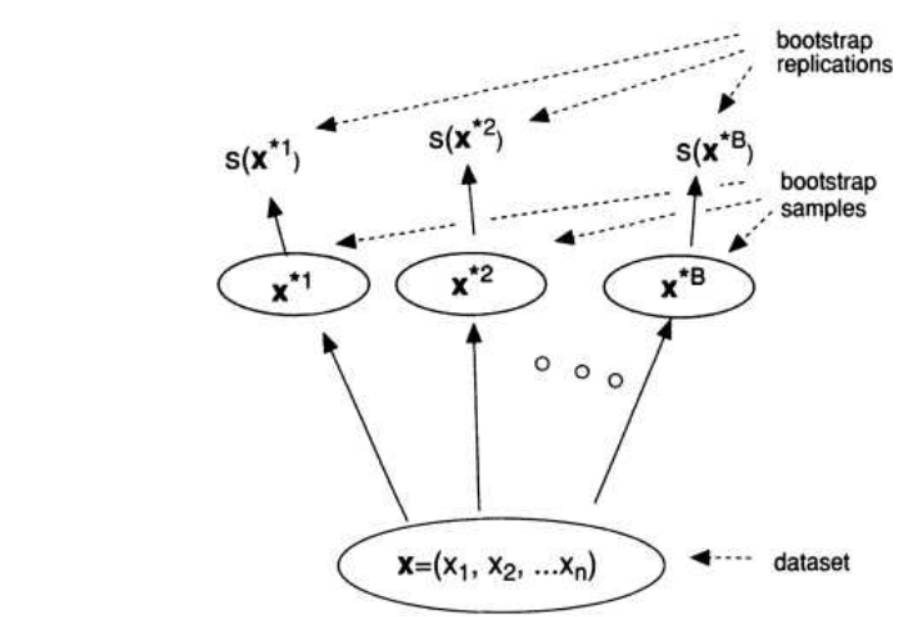
\includegraphics[width=0.5\linewidth]{ejemplo boots.png}
    \caption{}
    \label{fig:enter-label}
\end{figure}

Este método se utiliza para la estimación de las proporciones de pobreza. Farrell et al. (1997) proporcionan ajustes de Bootstrap para estimaciones empíricas del intervalo de Bayes de proporciones de área pequeña. También se usa técnicas de bootstrap paramétricos para la estimación del error cuadrático medio MSE de las EBP.

\subsection*{Monte Carlo}
A diferencia del método bootstrap los métodos de Monte Carlo generan simulaciones aleatorias basadas en una distribución de probabilidad conocida o asumida (según el comportamiento de los datos). Se basa en el uso de modelos probabilísticos para simular datos de manera repetida. Estos métodos son útiles en escenarios donde se puede definir una distribución teórica de los datos. Este método es últil para realizar aproximaciones sobre los EBP

\section*{Paquete emdi}

El paquete emdi se utiliza para para estimar y mapear indicadores regionales desagregados. Utiliza varios métodos de estimación, como la estimación directa, la mejor predicción empírica (EBP) y el modelo a nivel de área de Fay y Herriot. También incluye extensiones para datos seleccionados de manera informativa y modelos con errores de medición.
\textbf{Funciones principales:}
\begin{itemize}
    \item \textbf{Estimación directa, EBP y FH:} Métodos disponibles para cada función.
    \item \textbf{Visualización:} Funciones como 'map\_plot' y 'write.excel' para crear mapas y exportar resultados a Excel.
    \item \textbf{Evaluación del modelo:}Resúmenes y gráficos de diagnóstico para evaluar el modelo utilizado.
\end{itemize}

Ciertamente. Aquí tienes la traducción al español y en formato LaTeX de las secciones Usage, Arguments, Details y Value para las funciones `direct` y `ebp`:

Ciertamente. Aquí tienes la traducción al español y en formato LaTeX de las secciones Uso, Argumentos, Detalles y Valor para la función `fh`:

\subsubsection*{Uso}
\begin{verbatim}
direct(
  y,
  smp_data,
  smp_domains,
  weights = NULL,
  design = NULL,
  threshold = NULL,
  var = FALSE,
  boot_type = "naive",
  B = 50,
  seed = 123,
  X_calib = NULL,
  totals = NULL,
  custom_indicator = NULL,
  na.rm = FALSE
)
\end{verbatim}


\subsection*{Función ebp}

\subsubsection*{Uso}
\begin{verbatim}
ebp(
  fixed,
  pop_data,
  pop_domains,
  smp_data,
  smp_domains,
  L = 50,
  threshold = NULL,
  transformation = "box.cox",
  interval = "default",
  MSE = FALSE,
  B = 50,
  seed = 123,
  boot_type = "parametric",
  parallel_mode = ifelse(grepl("windows", .Platform$OS.type), "socket", "multicore"),
  cpus = 1,
  custom_indicator = NULL,
  na.rm = FALSE,
  weights = NULL,
  pop_weights = NULL,
  aggregate_to = NULL
)
\end{verbatim}


\subsection*{Función fh}

\subsubsection*{Uso}
\begin{verbatim}
fh(
  fixed,
  vardir,
  combined_data,
  domains = NULL,
  method = "reml",
  interval = NULL,
  k = 1.345,
  mult_constant = 1,
  transformation = "no",
  backtransformation = NULL,
  eff_smpsize = NULL,
  correlation = "no",
  corMatrix = NULL,
  Ci = NULL,
  tol = 1e-04,
  maxit = 100,
  MSE = FALSE,
  mse_type = "analytical",
  B = c(50, 0),
  seed = 123
)
\end{verbatim}

\section{Paquete survey}

El paquete survey en R es una herramienta diseñada para analizar datos de encuestas que han sido obtenidos mediante muestreo complejo, como los muestreos estratificados, por conglomerados, o con ponderaciones. Este paquete permite ajustar modelos estadísticos que tomen en cuenta la estructura del diseño de la encuesta, lo cual es crucial para obtener estimaciones correctas y evitar sesgos.

Principales funcionalidades del paquete survey:

\begin{itemize}
    \item Definir un diseño de encuesta: A través de la función svydesign, se puede especificar el tipo de diseño de muestreo, incluyendo ponderaciones, estratos, y conglomerados.
    \item Calcular estadísticas: Una vez definido el diseño, se pueden calcular estadísticas descriptivas, como medias, totales, proporciones y varianzas ajustadas por el diseño.
    \item  Modelos estadísticos: Permite ajustar modelos lineales y no lineales, como regresiones, para analizar la relación entre variables de la encuesta.
    \item  Estimaciones robustas: Las estimaciones producidas consideran la complejidad del muestreo, ajustando los errores estándar, los intervalos de confianza y las pruebas de hipótesis.
\end{itemize}

\subsection{Ejemplo básico de uso del paquete survey:}

\begin{verbatim}
Instalar y cargar el paquete
install.packages("survey")
library(survey)

# Cargar un dataset de ejemplo
data(api)

# Definir el diseño de la encuesta (muestreo estratificado)
dstrata <- svydesign(id = ~1, strata = ~stype, weights = ~pw, data = apistrat, fpc = ~fpc)

# Calcular la media de una variable ponderada por el diseño de la encuesta
mean_api00 <- svymean(~api00, dstrata)
print(mean_api00)

# Ajustar un modelo de regresión lineal usando el diseño de la encuesta
model <- svyglm(api00 ~ ell + meals, design = dstrata)
summary(model)

\end{verbatim}

svydesign: Define el diseño de muestreo, en este caso, un muestreo estratificado donde stype es la variable que indica el estrato, y pw son las ponderaciones.

svymean: Calcula la media ponderada de la variable api00, ajustada por el diseño de la encuesta.

svyglm: Ajusta un modelo de regresión lineal ponderado usando las variables ell y meals como predictoras, teniendo en cuenta el diseño de la encuesta.

\section*{Encuestas por muestreo}

Las encuestas por muestreo son una una técnica estadística que se utiliza para recopilar por medio de una muestra datos representativos de una población específica

\subsection*{logcv}
Según CEPAL:
\textbf{Coeficiente de variación (CV):} este elemento se emplea para evaluar estimaciones que no correspondan a proporciones ni razones entre 0 y 1. En ese sentido, la mayoría de las oficinas de estadísticas establecen que son datos “no publicables” aquellas estimaciones cuyo coeficiente de variación supera el 20\% (Gutiérrez y otros, 2020). El valor de aceptación que se 
recomienda para evaluar la fiabilidad puede situarse entre 15 y 20. Para evaluar estimaciones poco fiables se aconseja un umbral entre 25 y 30 y, en caso de que el coeficiente de variación sea mayor que 30, se recomienda clasificar la cifra como no fiable. 

\textbf{Coeficiente de variación logarítmico (CVLog):} este elemento se emplea para evaluar las estimaciones que correspondan a una proporción o razón entre 0 y 1. Según lo propuesto por Barnett-Walker y otros (2003), se recomienda utilizar un umbral del 17,5\% para considerar una estimación fiable cuando el tamaño de muestra efectivo es 60; en caso contrario, se recomienda calificar la cifra como poco fiable o no fiable, acorde a los umbrales establecidos en el punto 
7. Este umbral de aceptación puede modificarse de acuerdo con el valor de la función logarítmica del coeficiente de variación evaluada en p = 0,5 según los valores que puede tomar el tamaño de muestra efectivo.


\subsection*{grados de libertad}
\newpage
\section*{Ejemplo: Estimadores de Fay-herriot de incidencias de pobreza en R:}

El ejemplo a mostrar a continuación se encuentra en un informe de investigación titulado “Desagregación de datos en encuestas de hogares: Metodologías de estimación en áreas pequeñas”. Es parte de la “Serie Estudios Estadísticos” número 97, publicado por CEPAL.

Vamos a ilustrar cómo calcular estimadores de Fay-Herriot para las incidencias de pobreza, usando datos simulados sobre condiciones de vida en las provincias españolas, incluidos en el fichero de datos de R llamado \texttt{incomedata} del paquete de R \texttt{sae}. Este conjunto de datos incluye, para $n = 17119$ individuos ficticios que residen en las $D = 52$ provincias españolas, el nombre de la provincia donde reside (\texttt{provlab}), el código de la provincia (\texttt{prov}), el código de la comunidad autónoma (\texttt{ac}), el grupo de edad de 1 a 5 (\texttt{age}), la nacionalidad (\texttt{nat}, 1=si posee la española, 2=si no la posee), el nivel educativo (\texttt{educ}, de 0=menor de 16 años a 3=nivel universitario), la situación laboral (\texttt{labor}, donde 0=menor de 16 años, 1=ocupado, 2=desempleado y 3=inactivo), si está en cada grupo de edad, desde el grupo 2 hasta el 5 (\texttt{age2} hasta \texttt{age5}), si posee el nivel educativo 1 hasta 3 (\texttt{educ1} hasta \texttt{educ3}), si posee la nacionalidad española, si está ocupado, parado o inactivo, los ingresos netos equivalentes (\texttt{income}) y el peso muestral (\texttt{weight}). Calculamos los estimadores directos de HT para las incidencias de pobreza en las $D=52$ provincias españolas.

Después de instalar la librería \texttt{sae}, la cargamos, junto con el conjunto de datos \texttt{incomedata}, que contiene los datos muestrales, y el conjunto de datos \texttt{sizeprov}, que contiene los tamaños poblacionales de las provincias, $N_d$:

\begin{lstlisting}[language=R]
library(sae) 
data(incomedata) 
attach(incomedata) 
data(sizeprov) 
n<-dim(incomedata)[1]  # Tamano muestral total 
D <-length(unique(prov))      # Numero de provincias (areas o dominios) 
nd<-as.vector(table(prov))   # Tamanos muestrales de las provincias 
Nd<-sizeprov$Nd              # Tamanos poblacionales de las provincias 
\end{lstlisting}

Establecemos el umbral de pobreza, que se calcula como \texttt{0.6*median(income)} con los datos del año anterior, y construímos la variable poor, que es el indicador de tener ingresos por debajo del umbral de 
pobreza:  
\begin{lstlisting}[language=R]
z<-6557.143 
poor<-numeric(n) 
poor[income<z]<-1    
\end{lstlisting}
Finalmente, calculamos los estimadores directos de HT de las incidencias de pobreza en las provincias (promedios de la variable poor en las provincias), usando la función direct() incluyendo los pesos muestrales dados por la variable weight:  
\begin{lstlisting}[language=R]
povinc.dir.res<-direct(y=poor,dom=prov,sweight=weight,domsize=sizeprov[,-1]) 
print(povinc.dir.res,row.names=F) 
\end{lstlisting}
Se comprueba el supuesto de normalidad:
\begin{lstlisting}[language=R]
povinc.dir<-povinc.dir.res$Direct 
hist(povinc.dir,prob=TRUE,main="",xlab="HT estimators pov. 
incidence")
\end{lstlisting}

La forma de este histograma (no se incluye por brevedad) es algo asimétrica pero no se aleja demasiado de una densidad normal, lo cual es esperable puesto que se aplica el Teorema Central del límite a los estimadores directos de las áreas. 

A continuación, cargamos los conjuntos de datos con los tamaños poblacionales de las provincias 
y los mismos por grupos de nacionalidad, edad y estado laboral (algunos ya estaban cargados en los 
ejemplos anteriores): 

\begin{lstlisting}[language=R]
data(sizeprov) 
data(sizeprovnat) 
data(sizeprovage) 
data(sizeprovedu) 
data(sizeprovlab)  
\end{lstlisting}

Usamos estos tamaños poblacionales para calcular las proporciones de individuos en cada categoría dentro de cada provincia. Éstos serán nuestras variables explicativas en un modelo Fay-Herriot:  
\begin{lstlisting}[language=R]
Nd<-sizeprov[,3] 
Ndnat<-as.matrix(sizeprovnat[,-c(1,2)]) 
Ndage<-as.matrix(sizeprovage[,-c(1,2)]) 
Ndedu<-as.matrix(sizeprovedu[,-c(1,2)]) 
Ndlab<-as.matrix(sizeprovlab[,-c(1,2)]) 
Pdnat<-Ndnat/Nd 
Pdage<-Ndage/Nd 
Pdedu<-Ndedu/Nd 
Pdlab<-Ndlab/Nd 
# Matriz de diseno para modelo FH 
X<-cbind(const=rep(1,D),nat1=Pdnat[,1],Pdage[,3:5],Pdedu[,c(1,3)],Pdlab[,c(2,3)])
\end{lstlisting}

Llamamos a la función que calcula los estimadores FH de las incidencias de pobreza para las provincias, usando los estimadores directos HT obtenidos en el Ejemplo 1 y sus correspondientes varianzas muestrales: 

\begin{lstlisting}[language=R]
povinc.FH.res<-eblupFH(povinc.dir~X-1,vardir=povinc.dir.res$SD^2) 
povinc.FH<-povinc.FH.res$eblup     
\end{lstlisting}

Usando los coeficientes de regresión estimados obtenidos del ajuste del modelo Fay-Herriot, podemos calcular también estimadores sintéticos de regresión basados en el modelo a nivel de área: 
\begin{lstlisting}[language=R]
povinc.rsyn1<-X%*%povinc.FH.res$fit$estcoef[,1]
\end{lstlisting}

Aunque estos estimadores están basados en el estimador de los coeficientes de regresión obtenidos del ajuste del modelo Fay-Herriot y no del modelo sintético, también son estimadores sintéticos pues no consideran heterogeneidad entre áreas no explicada por las variables auxiliares 
consideradas. Además, los estimadores de los coeficientes de regresión obtenidos bajo ambos modelos, usando las mismas variables auxiliares, son asintóticamente equivalentes. Por tanto, para un número de áreas grande, ambos serán muy similares. Como los estimadores FH son estimadores compuestos entre los directos y los sintéticos de regresión, calculamos los pesos que se dan a los estimadores directos en la composición: 

\begin{lstlisting}[language=R]
gammad<-povinc.FH.res$fit$refvar/(povinc.FH.res$fit$refvar+povinc.dir.res$SD^2) 
\end{lstlisting}

\begin{lstlisting}
> summary(gammad) 
   Min. 1st Qu.  Median    Mean 3rd Qu.    Max. 
 0.4537  0.7182  0.8108  0.7906  0.8977  0.9477 
\end{lstlisting}

Vemos que, a diferencia de los estimadores SSC, en este caso el peso que se le otorga al estimador directo no es igual a uno para ninguna provincia, aunque sí toma valores cercanos a uno para algunas provincias.  Ahora comparamos gráficamente las estimaciones FH con las directas HT y sintéticas (llamadas RSYN1) para cada provincia. Las provincias (en el eje) se ordenan de menor a mayor tamaño muestral, e indicamos los tamaños muestrales de éstas en el eje: 

\begin{lstlisting}[language=R]
o<-order(nd) 
k<-6 
M<-max(povinc.dir,povinc.FH,povinc.rsyn1) 
m<-min(povinc.dir,povinc.FH,povinc.rsyn1) 
plot(1:D,povinc.dir[o],type="n",ylim=c(m,M+(M-m)/k),xlab="Province",ylab="Estimator", 
xaxt="n") 
points(1:D,povinc.dir[o],type="b",col=1,lty=1,pch=1,lwd=2) 
points(1:D,povinc.FH[o],type="b",col=4,lty=4,pch=4,lwd=2) 
points(1:D,povinc.rsyn1[o],type="b",col=3,lty=3,pch=3,lwd=2) 
axis(1, at=1:D, labels=nd[o]) 
legend(1,M+(M-m)/k,legend=c("DIR","FH","RSYN1"),ncol=3,col=c(1,4,3),lwd=rep(2,3), 
lty=c(1,4,3),pch=c(1,4,3)) 
\end{lstlisting}
Finalmente, estimamos el ECM de los estimadores FH, llamando a la función mseFH(), calculamos los CVs estimados y graficamos los ECMs junto a las varianzas de los estimadores directos:  
\begin{lstlisting}[language=R]
povinc.FH.mse.res<-mseFH(povinc.dir~X-1,vardir=povinc.dir.res$SD^2) 
povinc.FH.mse<-povinc.FH.mse.res$mse 
povinc.FH.cv<-100*sqrt(povinc.FH.mse)/povinc.FH 
M<-max(povinc.dir.var,povinc.FH.mse) 
m<-min(povinc.dir.var,povinc.FH.mse) 
plot(1:D,povinc.dir.cv[o],type="n",ylim=c(m,M+(M-m)/k),xlab="Province",ylab="CV",xaxt="n") 
points(1:D,povinc.dir.var[o],type="b",col=1,lty=1,pch=1,lwd=2) 
points(1:D,povinc.FH.mse[o],type="b",col=4,lty=4,pch=4,lwd=2) 
axis(1, at=1:D, labels=nd[o]) 
legend(1,M+(M-m)/k,legend=c("DIR","FH"),ncol=3,col=c(1,4),lwd=rep(2,2),lty=c(1,4),pch=c(1,4))
\end{lstlisting}



\begin{figure}[H]
    \centering
    \begin{subfigure}[b]{0.45\textwidth}
        \centering
        \includegraphics[width=\textwidth]{estimaciones directas y FH y MSE.png}
        \label{fig:imagen1}
    \end{subfigure}
    \begin{subfigure}[b]{0.45\textwidth}
        \centering
        \includegraphics[width=\textwidth]{estimaciones directas y FH.png}
        \label{fig:imagen2}
    \end{subfigure}
    \caption{Estimaciones FH, directas HT y RSYN1 de las incidencias de pobreza para las provincias (izquierda), y ECMs estimados de los estimadores FH y directos HT (derecha) 
    (En proporciones)}
    \label{fig:imagenes_paralelas}
\end{figure}

De nuevo, podemos ver en el Gráfico 6 (izquierda) que los estimadores sintéticos de regresión toman valores similares para todas las provincias, a diferencia de los estimadores directos, que varían más a lo largo de éstas. Los estimadores FH se acercan a los directos, pero al mismo tiempo toman información prestada de las demás provincias a través de los estimadores sintéticos, especialmente para las provincias de menor tamaño muestral (parte izquierda del gráfico). Aunque en este ejemplo las variables auxiliares 
consideradas no sean muy potentes, el Gráfico 6 (derecha) sugiere que los estimadores FH son más eficientes que los directos. 

Finalmente, vamos a comparar los CVs estimados para los estimadores HT, GREG y FH para las 5 
provincias con menores tamaños muestrales: 

\begin{lstlisting}[language=R]
compardirFH<-data.frame(povinc.dir.cv,povinc.greg.cv,povinc.FH.cv) 
selprov<-o[1:5] 
compardirFH[selprov,]    
\end{lstlisting}

\begin{lstlisting}
> compardirFH[selprov,]
   povinc.dir.cv povinc.FH.cv
42      99.97815     49.47213
5       46.35946     34.00564
40      25.33449     22.13933
34      23.80085     18.69105
44      24.57017     21.32242
\end{lstlisting}

Podemos ver la reducción en los CVs que consiguen los estimadores FH en comparación con los estimadores directos HT para las cuatro provincias de menores tamaños muestrales, y las ganancias son considerables para las dos provincias de tamaños muestrales más pequeños. 





\begin{thebibliography}{3}

\bibitem{Libro}
Morales, D., Esteban, M. D., Pérez, A., \& Hobza, T. (2021). A Course on Small Area Estimation and Mixed Models: Methods, Theory and Applications in R. Springer. \url{https://doi.org/10.1007/978-3-030-63757-6} 

\bibitem{informe}
Molina, I. (2021). Desagregación de datos en encuestas de hogares: Metodologías de estimación en áreas pequeñas. Naciones Unidas CEPAL.



\end{thebibliography}
\end{document}